\chapter{Data export}

InVesalius can export data in different formats, such as OBJ, STL and others, to be used in other software.

The menu to export data is located in the left panel of InVesalius, inside item \textbf{4. Export data} (displayed below in Figure~\ref{fig:data_export}). If the menu is not visible, double-click with the \textbf{left} mouse button to expand the item.

\begin{figure}[!htb]
\centering
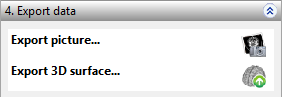
\includegraphics[scale=0.8]{painel_data_export_en.png}
\caption{Menu to export data}
\label{fig:data_export}
\end{figure}

\section{Surface}

To export a surface, select it from the data menu as shown in Figure~\ref{fig:data_export_selection}.

\newpage

\begin{figure}[!htb]
\centering
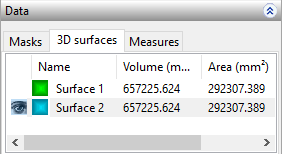
\includegraphics[scale=0.7]{painel_data_export_selection_en.png}
\caption{Select surface to be exported}
\label{fig:data_export_selection}
\end{figure}

Next, click on the icon shown in Figure~\ref{fig:surface_export_original}.

\begin{figure}[!htb]
\centering

\includegraphics[scale=0.2]{surface_export_original}
\caption{Shortcut to export surface}
\label{fig:surface_export_original}
\end{figure}

When the file window displays (as shown in Figure~\ref{fig:export_data_window}), type the file name and select the desired exported format. Finally, click \textbf{Save}.

\begin{figure}[!htb]
\centering
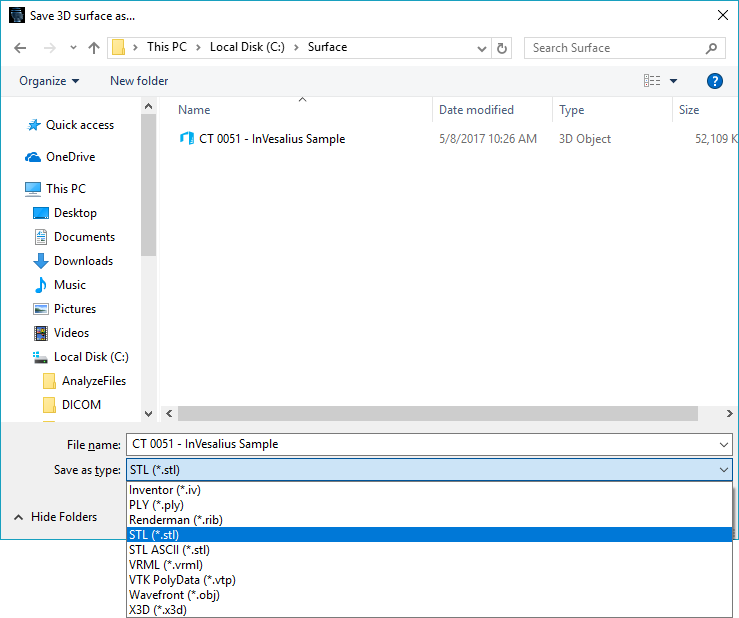
\includegraphics[scale=0.4]{export_surface_en.png}
\caption{Window to export surface}
\label{fig:export_data_window}
\end{figure}

Files formats avaiable for exportation are listed in table~\ref{tab:files_export_list}:

\begin{table}[h]
\centering
\caption{File formats exported by InVesalius}
\begin{tabular}{lcc}\\
\hline % este comando coloca uma linha na tabela
Format & Extension\\
\hline
\hline
Inventor & .iv\\
Polygon File Format & .ply\\
Renderman & .rib\\
Stereolithography (formato binário)& .stl\\
Stereolithography (formato ASCII) & .stl\\
VRML & .vrml\\
VTK PolyData & .vtp\\
Wavefront & .obj\\
\hline
\end{tabular}
\label{tab:files_export_list}
\end{table} 


\section{Image}

Images exhibited in any orientation (axial, coronal, sagittal and 3D) can be exported. To do so, \textbf{left-click} on the shortcut shown in Figure~\ref{fig:menu_save_image_window} and select the sub-window related to the target image to be exported.

\begin{figure}[!htb]
\centering
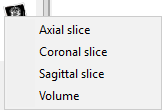
\includegraphics[scale=0.5]{menu_save_image_window_en.png}
\caption{Menu to export images}
\label{fig:menu_save_image_window}
\end{figure}

On the window shown (Figure~\ref{fig:save_image_window}), select the desired file format, then click \textbf{Save}.

\begin{figure}[!htb]
\centering
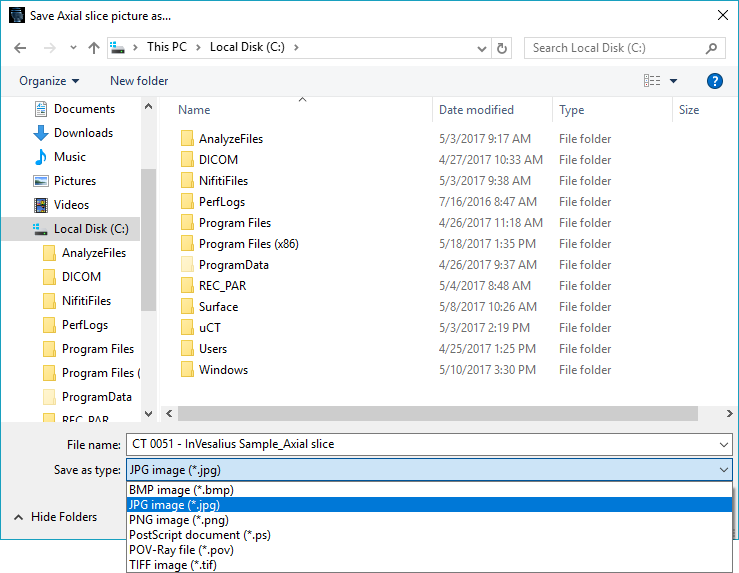
\includegraphics[scale=0.4]{export_bmp_en.png}
\caption{Window to export images}
\label{fig:save_image_window}
\end{figure}
